% !TEX engine = lualatex
\documentclass[aspectratio=169,usepdftitle=false]{fireshonks}

%%%%%%%%%%%%%%%%%%%%%
% PAQUETES
%%%%%%%%%%%%%%%%%%%%%

\setdefaultlanguage{english}
\setotherlanguage{german}
\usepackage{tikz}
\usetikzlibrary{arrows.meta, matrix, shapes.geometric, overlay-beamer-styles}
\usepackage[german]{datetime2}
\usepackage{subcaption}
\usepackage{import}
\usepackage{siunitx}
\usepackage{fontawesome5}
\usepackage{emoji}
\sisetup{mode=text, per-mode=symbol}
\captionsetup{font+=scriptsize,justification=centering}
\usepackage{tabularray}
\UseTblrLibrary{booktabs}
\usepackage{qrcode}

%%%%%%%%%%%%%%%%%%%%%
% TEMPLATE
%%%%%%%%%%%%%%%%%%%%%
% Title graphics: BG + logo of the conference
\titlegraphic{
  \begin{tikzpicture}[remember picture, overlay]
    \mode<beamer>{\scoped[on background layer]\node [centered,opacity=0.4] at (current page.center) {
\includegraphics[width=\pagewidth,height=\pageheight,keepaspectratio]{frontmatter/cropped-Try_This_At_Home-1920x1080-1.png}};}
    \scoped[on background layer]\node [below left] at (current page.north east) {
\includegraphics[height=4em,keepaspectratio]{frontmatter/annie-shenanigans}};
    % Background: FireShonks  \\
    \scoped[on background layer]\node [above right,align=left,font=\tiny\itshape] at (current page.south west) {
      Seal: \href{https://lethalbit.net}{Aki Van Ness}, CC-BY-SA-4.0
    };
  \end{tikzpicture}
}

%%%%%%%%%%%%%%%%%%
% METADATA
%%%%%%%%%%%%%%%%%%

\title{The Unsung Heroes of Imaging}
\author{amyspark}
\date{\DTMdate{2023-12-27}}

\addbibresource{bibliography.bib}

\begin{document}
\maketitle

\begin{frame}{About me}
    \begin{itemize}[<*>]
        \item Upstreamer \& Compiler Breaker at Centricular
              \begin{itemize}[<*>]
                  \item Fine purveyors of Free and Open Source Software consulting
                  \item Maintainers of the GStreamer multimedia framework
              \end{itemize}
        \item Colour spaces, SIMD, build systems... curses are my specialty \emoji{woman-mage}
        \item Occasional contributor to a lot of projects
    \end{itemize}
\end{frame}
\begin{frame}{Motivation}
    \begin{itemize}
        \item Most of you may understand terms like \enquote{JPG picture}, \enquote{PNG}, even \enquote{TIFF}...
        \item Watching TV? You may have heard about \enquote{PAL}, \enquote{NTSC}, \enquote{SECAM}
        \item How do we store and broadcast colour images?
    \end{itemize}
\end{frame}

\begin{frame}{Motivation}
    \begin{itemize}
        \item Why is a JPEG picture so small compared to PNG, TIFF, RAW...?
        \item How can we watch \emoji{cat} videos on phones?
        \item How were we able to watch colour TV before the PC era?
        \item \emoji{woman-mage} there's a \emph{luma-chroma colour space} involved to compress them!
        \item Lots of background to cover, includes a bit of HDR too!
    \end{itemize}
\end{frame}
\begin{frame}{Scope}
    \tableofcontents
\end{frame}
\section{Introduction}
\begin{frame}{How are colours specified?}
    Colours are specified as coordinates in a \emph{colour space}.
    \begin{itemize}[<+(1)->]
        \item $n$-dimensional geometrical model
        \item Light stimuli (colours) $\leftrightarrow$ vector coordinates
        \item If you've taken a picture, or browsed the web, you've run across them
              \begin{itemize}
                  \item The sRGB colour space powers most consumer content nowadays
              \end{itemize}
    \end{itemize}
\end{frame}
\begin{frame}{Colour spaces as a mathematical construct}
    \begin{itemize}
        \item Coordinate system
        \item A subspace within that system
        \item A mapping function from a \emph{supported} colour to a single point inside the subspace
        \item The set of supported colours is the colour space's \emph{gamut}
    \end{itemize}
\end{frame}
\begin{frame}{Formal definition of a colour space}
    \begin{columns}<.->
        \begin{column}<.->{.7\textwidth}
            \begin{itemize}
                \item Two sets of components:
                      \begin{enumerate}
                          \item Three independent, reference stimuli: \emph{primaries}
                          \item Colour of the light source: white point or \emph{illuminant}
                      \end{enumerate}
                \item These components are represented by their \emph{chromaticity} coordinates
                \item Plotting them in \emph{chromaticity diagrams} reveals the space's gamut
            \end{itemize}
        \end{column}
        \begin{column}<.->{.3\textwidth}
            \begin{figure}
                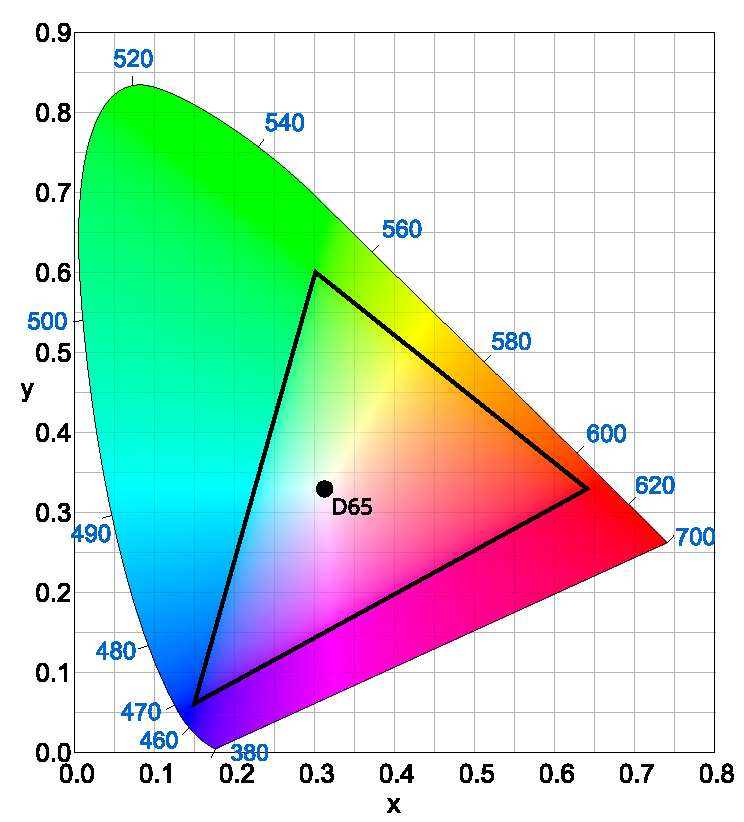
\includegraphics[width=\columnwidth,keepaspectratio]{figures/bt709.pdf}
                \caption*{The colour space of ITU-R BT.709 \parencite*{BT709}. Source: \href{https://commons.wikimedia.org/wiki/File:CIExy1931_Rec_709.svg}{GrandDrake}, \href{http://creativecommons.org/licenses/by-sa/3.0/}{CC BY-SA 3.0}, via Wikimedia Commons}
            \end{figure}
        \end{column}
    \end{columns}
\end{frame}
\begin{frame}{How are colours stored and transmitted?}
    From abstract to concrete:
    \begin{enumerate}
        \item Colour model \emph{type}
        \item Colour \emph{model}
        \item Colour \emph{space}
        \item Colour \emph{encoding}
    \end{enumerate}
\end{frame}
\begin{frame}{Colour model types}
    How they represent colours with their primaries \autocite{allen23}:
    \begin{itemize}
        \item \emph{Additive} colour models mix light stimuli to form colours
              \begin{itemize}
                  \item The most well known example is RGB
                  \item Three primaries: red, green, blue
                  \item Three coordinates: $(r, g, b)$ for each channel
                  \item HSL, HSI, HSV are linear transformations of RGB and are used in web dev
              \end{itemize}
        \item \emph{Subtractive} colour models absorb light stimuli to form colours
              \begin{itemize}
                  \item The most well known example is CMYK (cyan, magenta, yellow, and black ink)
              \end{itemize}
    \end{itemize}
\end{frame}
\begin{frame}{Example: the sRGB colour space}
    \emph{sRGB} (\enquote{standard RGB}) powers most consumer content nowadays.
    \begin{itemize}
        \item Type: Additive
        \item Model: RGB
        \item Definition: ISO/IEC 61966-2-1 \parencite*{srgb2002}
        \item Encoding: Most standards provide conversion formulae for the intended bit depth
              \begin{itemize}
                  \item This one is designed for \emph{8-bit unsigned integer}
              \end{itemize}
    \end{itemize}
\end{frame}
\begin{frame}{Colour management}
    \begin{itemize}
        \item In the analog era, there was a single colour space
              \begin{itemize}
                  \item Standardized in Recommendations from the International Telecommunications Union
                  \item e.g. ITU.R BT-709 \parencite*{BT709} for digital SD TV content
                  \item There were variations in broadcasting standards -- we'll cover these later
              \end{itemize}
        \item In the digital era, we need \emph{colour management systems}
    \end{itemize}
\end{frame}
\begin{frame}{Colour management}
    \begin{itemize}
        \item Modern colour management systems follow the International Colour Consortium's framework \autocite{allen}
        \item \emph{Open-loop} colour management
        \item Calculations are done in a \emph{profile connection space} (PCS)
              \begin{itemize}
                  \item Intermediate, device-independent colour space
                  \item Primaries and illuminant are defined in this colour space
              \end{itemize}
        \item Conversions to/from each device $\equiv$ \emph{transformation} from/to the PCS
              \begin{itemize}
                  \item (note the inverted directions)
              \end{itemize}
    \end{itemize}
\end{frame}
\begin{frame}{Open-loop colour management}
    \begin{figure}
        \begin{tikzpicture}[
                node distance=3em and 5em,
                device/.style={align=center, font=\Large},
                pcs/.style={circle, text width=3em, align=center, draw},
                transform/.style={->,shorten >=1pt,>=Latex,semithick}
            ]
            \node (i1) [device] {\emoji{camera}};
            \node (i2) [device, below=of i1] {\emoji{video-camera}};
            \node (i3) [device, below=of i2] {\emoji{movie-camera}};
            \node (pcs) [pcs, right=of i2] {PCS};
            \node (d1) [device, above=of pcs] {\emoji{desktop-computer}};
            \node (d2) [device, below=of pcs] {\emoji{mobile-phone}};
            \node (o1) [device, above right=of pcs] {\emoji{printer}};
            \node (o2) [device, below right=of pcs] {\emoji{printer}};

            \draw[transform] (i1) -- (pcs) node [midway, visible on=<2->] {\emoji{arrows-counterclockwise}};
            \draw[transform] (i2) -- (pcs) node [midway, visible on=<2->] {\emoji{arrows-counterclockwise}};
            \draw[transform] (i3) -- (pcs) node [midway, visible on=<2->] {\emoji{arrows-counterclockwise}};
            \draw[transform] (i1) -- (pcs) node [midway, visible on=<2->] {\emoji{arrows-counterclockwise}};
            \draw[transform] (pcs) -- (d1) node [midway, visible on=<2->] {\emoji{arrows-counterclockwise}};
            \draw[transform] (pcs) -- (d2) node [midway, visible on=<2->] {\emoji{arrows-counterclockwise}};
            \draw[transform] (pcs) -- (o1) node [midway, visible on=<2->] {\emoji{arrows-counterclockwise}};
            \draw[transform] (pcs) -- (o2) node [midway, visible on=<2->] {\emoji{arrows-counterclockwise}};
        \end{tikzpicture}

        \caption*{Adapted from \textcite[viii]{icc}}
    \end{figure}
\end{frame}
\begin{frame}{The ICC colour management architecture}
    Four key components:
    \begin{enumerate}[<+(1)->]
        \item The PCS
        \item The \emph{colour management module}
              \begin{itemize}
                  \item A software library that performs all the colour conversions
                  \item Usually embedded on your OS, there are also vendor offerings available
              \end{itemize}
        \item The device profiles
              \begin{itemize}
                  \item Contain the data to transform between PCS and the device's colour space
                  \item \emoji{woman-mage} our spaces are here
              \end{itemize}
        \item Rendering \emph{intents}
              \begin{itemize}
                  \item Exact matches between spaces may not be possible: \emph{out-of-gamut} colours
                  \item The CMS needs to \emph{predictably} account for this
              \end{itemize}
    \end{enumerate}
\end{frame}
\begin{frame}{The ICC colour management architecture}
    \begin{center}
        Interested? Watch my talk at DiVOC!

        \qrcode[hyperlink,height=4\baselineskip]{https://media.ccc.de/v/divoc_bb3-48292-the-last-frontier-on-icc-profiles}

        \url{https://media.ccc.de/v/divoc_bb3-48292-the-last-frontier-on-icc-profiles}
    \end{center}
\end{frame}
\section{What are these spaces?}
\begin{frame}{Reasoning}
    \begin{center}
        Digital encoding of colour signals for transmission (TV, streaming, etc.)
    \end{center}

    \uncover<+(1)->{What does it need to cover? \autocite{tooms}}
    \begin{enumerate}[<+(1)->]
        % Tooms 14.2.1
        \item Retaining colour balance
              \begin{itemize}
                  \item Colour drifts between different cameras? \emoji{pleading-face}
                  \item Colour drifts between different screens? \emoji{pleading-face}
              \end{itemize}
        \item Preserving the lightness information
              \begin{itemize}
                  \item Our eyes are most sensitive to light, not colour itself
              \end{itemize}
        \item Efficiency of the colour signal(s)
              \begin{itemize}
                  \item e.g. a single 1080p frame, 8-bit RGB uncompressed, is \SI{170}{\mega\byte}
                  \item How much of this space/bandwidth is actually needed?
              \end{itemize}
    \end{enumerate}
\end{frame}
\begin{frame}{Light? Colour?}
    \begin{itemize}
        \item Representing faithfully the response of the eye to light stimuli
        \item Colour information is split into two kinds of components:
              \begin{enumerate}
                  \item Luma
                        \begin{itemize}
                            \item \emph{Grayscale}, \emph{lightness}, etc.
                            \item Represents the luminosity information of the image
                        \end{itemize}
                  \item Chroma
                        \begin{itemize}
                            \item Represents the colours themselves
                        \end{itemize}
              \end{enumerate}
    \end{itemize}
\end{frame}
\begin{frame}{Luma? Luminance?}
    Before going on, we need to keep in mind that image transmission involves \emph{gamma correction} \autocite{tooms}.
    \begin{itemize}
        \item Formally called:
              \begin{enumerate}
                  \item \emph{Opto-electric transfer function} (OETF) for the digitalization of the scene
                  \item \emph{Electro-opto transfer function} (EOTF) for the display of the image
              \end{enumerate}
        \item Accounts for the non-linearity on image sensors and display devices
    \end{itemize}
\end{frame}
\begin{frame}{Gamma correction}
    Let's assume that all devices handle the sRGB colour space:
    \begin{figure}
        \centering
        \begin{tikzpicture}[
                node distance=2em and 5em,
                device/.style={align=center, font=\Large},
                pcs/.style={circle, text width=3em, align=center, draw},
                eotf/.style={->,shorten >=1pt,>=Latex,semithick,Red},
                transform/.style={->,shorten >=1pt,>=Latex,semithick},
                oetf/.style={->,shorten >=1pt,>=Latex,semithick,orange}
            ]
            \node (i1) [device] {\emoji{camera}};
            \node (i2) [device, below=of i1] {\emoji{video-camera}};
            \node (i3) [device, below=of i2] {\emoji{movie-camera}};
            \node (rgbi) [right=of i2]{RGB};
            \node (pcs) [pcs, right=of rgbi] {PCS};
            \node (rgbo) [right=of pcs] {RGB};
            \node (o) [right=of rgbo] {};
            \node (o1) [device, above=1em of o] {\emoji{mobile-phone}};
            \node (o2) [device, above=of o1] {\emoji{desktop-computer}};
            \node (o3) [device, below=1em of o] {\emoji{television}};
            \node (o4) [device, below=of o3] {\emoji{dvd}};

            \draw[oetf] (i1) -- (rgbi) node [midway, visible on=<2->] {\emoji{orange-circle}};
            \draw[oetf] (i2) -- (rgbi) node [midway, visible on=<2->] {\emoji{orange-circle}};
            \draw[oetf] (i3) -- (rgbi) node [midway, visible on=<2->] {\emoji{orange-circle}};
            \draw[transform] (rgbi) -- (pcs) node [midway, visible on=<3->] {\emoji{arrows-counterclockwise}};
            \draw[transform] (pcs) -- (rgbo) node [midway, visible on=<3->] {\emoji{arrows-counterclockwise}};
            \draw[eotf] (rgbo) -- (o1) node [midway, visible on=<4->] {\emoji{red-square}};
            \draw[eotf] (rgbo) -- (o2) node [midway, visible on=<4->] {\emoji{red-square}};
            \draw[eotf] (rgbo) -- (o3) node [midway, visible on=<4->] {\emoji{red-square}};
            \draw[eotf] (rgbo) -- (o4) node [midway, visible on=<4->] {\emoji{red-square}};

            \node [anchor=top, below=1em of pcs]{
                \small
                \begin{tblr}{colspec={cl}}%
                    \onslide<2->{\emoji{orange-circle}}           & \onslide<2->{OETF}                      \\
                    \onslide<3->{\emoji{arrows-counterclockwise}} & \onslide<3->{CMS transform to/from PCS} \\
                    \onslide<4->{\emoji{red-square}}              & \onslide<4->{EOTF}                      \\
                \end{tblr}
            };
        \end{tikzpicture}
    \end{figure}
\end{frame}
\begin{frame}{Luma/chroma v. luminance/chrominance}
    \begin{itemize}
        \item \emph{Luma} and \emph{chroma} mean gamma-corrected channels
              \begin{itemize}
                  \item $'$ attached to the variable name
                  \item It's usually written in the luminosity channel only
                  \item e.g. $Y'CbCr$ (one of the spaces we'll cover later) consumes gamma-corrected RGB
              \end{itemize}
        \item \emph{Luminance} and \emph{chrominance} mean linear (uncorrected) channels
              \begin{itemize}
                  \item e.g. $YCbCr$ consumes linear RGB, and will result in washed colours if fed gamma-corrected RGB
              \end{itemize}
    \end{itemize}
\end{frame}
\begin{frame}{Why all this baggage?}
    \begin{itemize}
        \item Preserving colour balance is \emph{essential}
        \item Errors in luma are very noticeable to the human eye
        \item Errors in chroma? not so much
        \item Codecs can drop spatial resolution \emph{and} lossily compress the colour data!
              \begin{itemize}
                  \item Less bandwidth/storage required
                  \item Faster transmission rates
                  \item e.g. a single 1080p frame, 8-bit RGB uncompressed, is \SI{170}{\mega\byte}
                  \item But you can squeeze it to less than a MB!
                  \item JPEG, H.264, HEVC, VP9, AV1... \emoji{clamp}\emoji{clamp}\emoji{clamp}
              \end{itemize}
        \item The process is known as \emph{chroma subsampling}
    \end{itemize}
\end{frame}
\begin{frame}{Chroma subsampling}
    \begin{figure}
        \centering
        \def\svgwidth{.6\textwidth}
        \subimport{figures}{Common_chroma_subsampling_ratios.pdf_tex}
        \caption*{Source: \href{https://commons.wikimedia.org/wiki/File:Common_chroma_subsampling_ratios.svg}{Stevo88}, Public Domain, via Wikipedia Commons}
    \end{figure}
\end{frame}
\section{Examples}
\begin{frame}{How's a luma-chroma space defined?}
    \begin{center}
        \emph{Transformations} of existing colour spaces
    \end{center}
    \begin{itemize}
        \item Base colour space
        \item Transformation function
              \begin{itemize}
                  \item Usually (not always \emoji{wink}) a linear transformation of the source space
              \end{itemize}
        \item Transfer functions, where applicable
    \end{itemize}
\end{frame}
\begin{frame}{Y'IQ}
    \begin{columns}<.->
        \begin{column}<.->{.7\textwidth}
            \begin{itemize}
                \item Created in 1953 for the NTSC analog broadcasting standard
                \item The oldest luma-chroma space in the imaging field
                \item ITU.R BT.470-6 \parencite*{BT470}, superseded by BT.1700-0 \parencite*{BT1700}
                \item $(R', G', B')$ pixel $\rightarrow$ $(Y', I, Q)$ signal values
                \item $Y'$ is the \emph{luma} signal
                      \begin{itemize}
                          \item Intuitively, our eyes are most sensitive to $G$
                          \item $G$ is a major contributor to the luminance value
                          \item $R$ and $B$ have smaller contributions
                      \end{itemize}
                \item $I$ and $Q$ together form the \emph{chroma} signal
                      \begin{itemize}
                          \item Complementary \emph{colour difference} signals
                      \end{itemize}
            \end{itemize}
        \end{column}
        \begin{column}<1->{.3\textwidth}
            \begin{figure}
                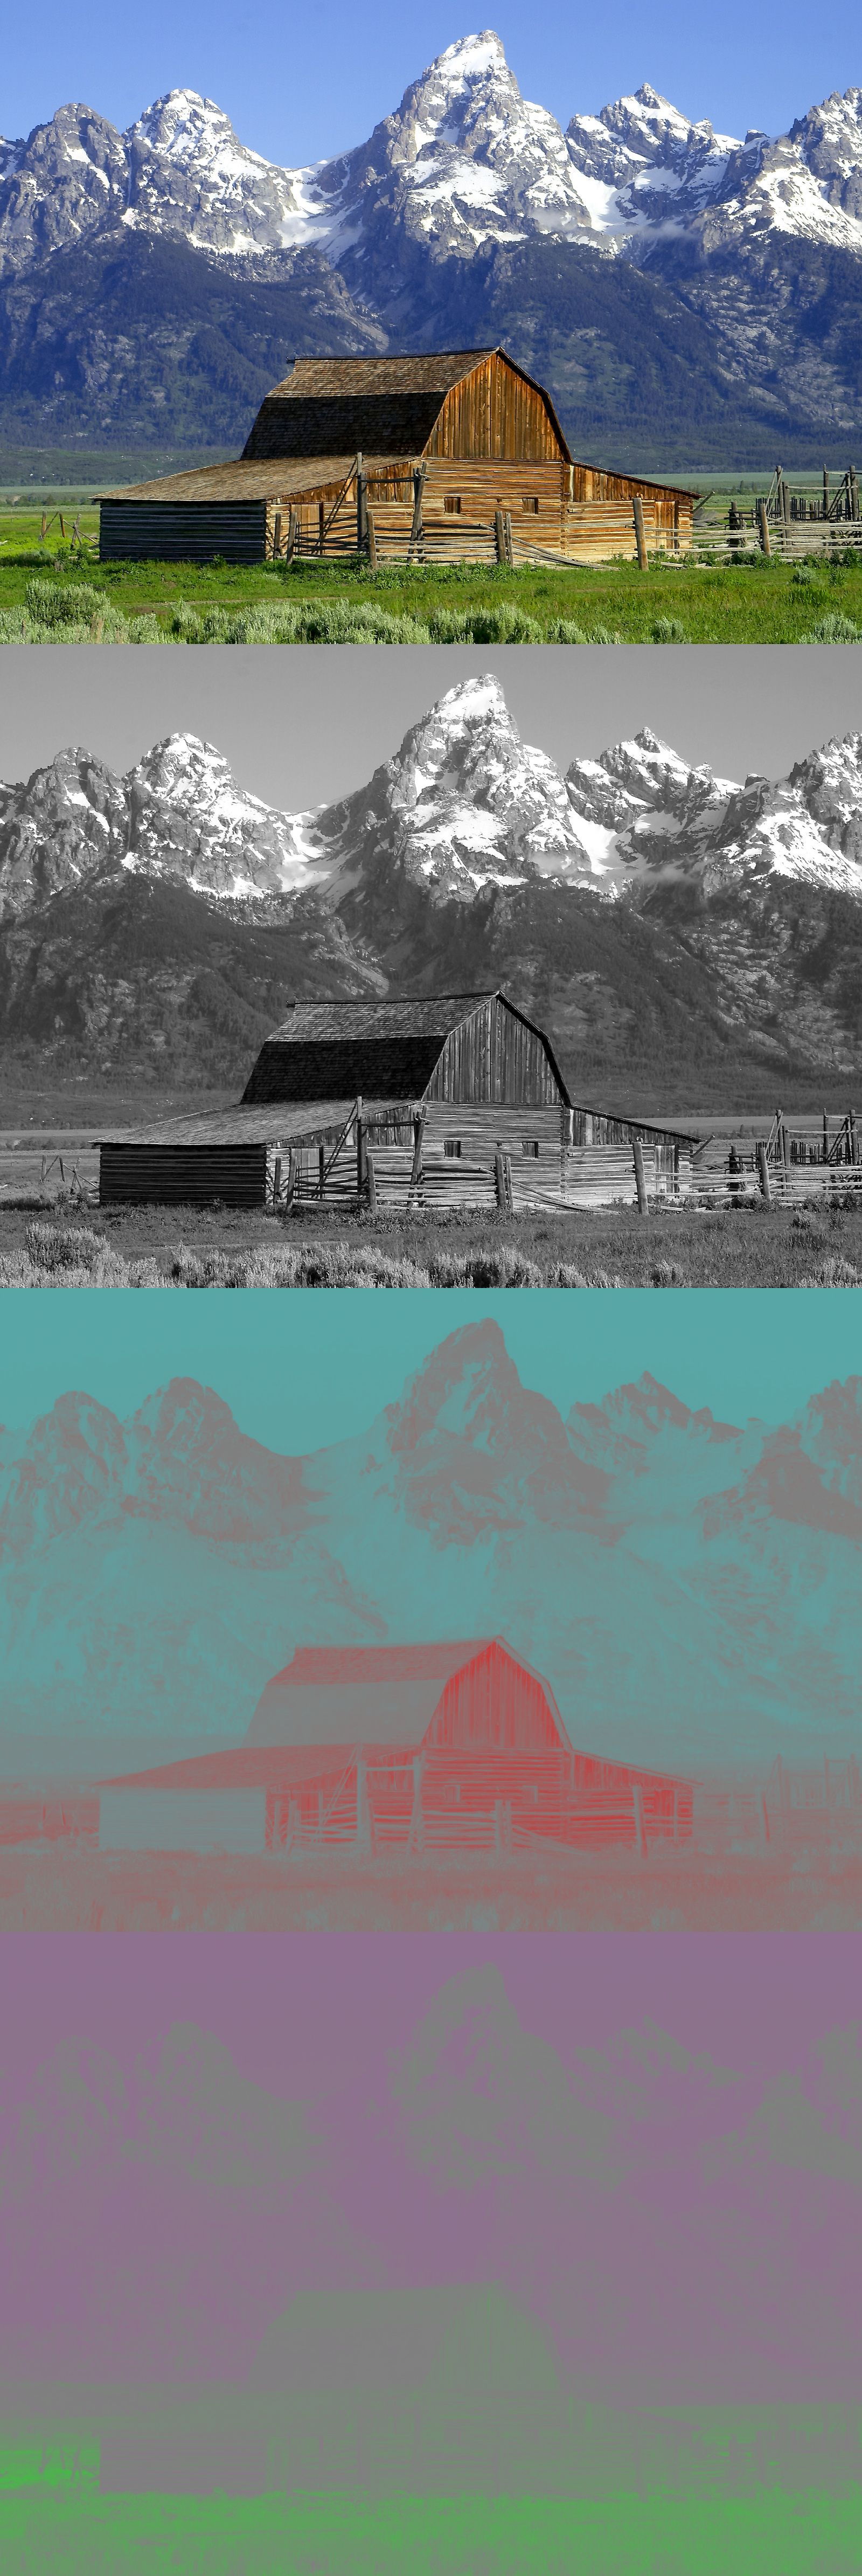
\includegraphics[height=10\baselineskip,keepaspectratio]{figures/YIQ_components.jpg}
                \caption*{Source: \href{https://commons.wikimedia.org/wiki/File:YIQ_components.jpg}{(3ucky(3all}, CC-BY-SA 3.0, via Wikimedia Commons}
            \end{figure}
        \end{column}
    \end{columns}
\end{frame}
\begin{frame}{Y'IQ: BT.1700-0}
    \begin{itemize}
        \item Targets standard definition, analog transmissions
        \item Targets a very old (CIE 1931) illuminant \emph{C}
        \item However, quickly obsoleted with the invention of PAL
        \item At the time, NTSC needed expensive circuitry to stabilize the signal
    \end{itemize}

    \uncover<+->{
        \begin{align}
            Y' & = 0.299R' + 0.587G' + 0.114B'  \\
            I  & = 0.596R' - 0.275G' - 0.322 B' \\
            Q  & = 0.211R' - 0.523G' + 0.312B'
        \end{align}
    }
\end{frame}
\begin{frame}{Y'IQ: gamma correction}
    \begin{itemize}
        \item Y'IQ takes/returns a gamma-corrected RGB signal
        \item The OETF relates the input luminance $L$ to the electrical signal $E$: \begin{equation}
                  \small
                  E = \begin{cases}
                      (1.099L^{0.045} - 0.099) & 0.018 < L \leq 1.00 \\
                      4.500L                   & 0 \leq L \leq 0.018
                  \end{cases}
              \end{equation}
        \item The EOTF relates the electrical signal $E$ to the output luminance $L$: \begin{equation}
                  \small
                  L = \begin{cases}
                      \frac{E + 0.099}{1.099}^\frac{1}{0.4500} & 0.0812 < E \leq 1.00 \\
                      \frac{E}{4.500}                          & 0 \leq L \leq 0.0812
                  \end{cases}
              \end{equation}
    \end{itemize}
\end{frame}
\begin{frame}{Y'DbDr}
    \begin{columns}<.->
        \begin{column}<.->{.7\textwidth}
            \begin{itemize}
                \item Entered use in France in 1967
                \item Objective: fix NTSC's need for phase signal adjustment
                \item $(R', G', B')$ pixel $\rightarrow$ $(Y', Db, Dr)$ signal values
                \item $Y'$ is the \emph{luma} signal
                \item $Db$ and $Dr$ together form the \emph{chroma} signal
            \end{itemize}
        \end{column}
        \begin{column}<1->{.3\textwidth}
            \begin{figure}
                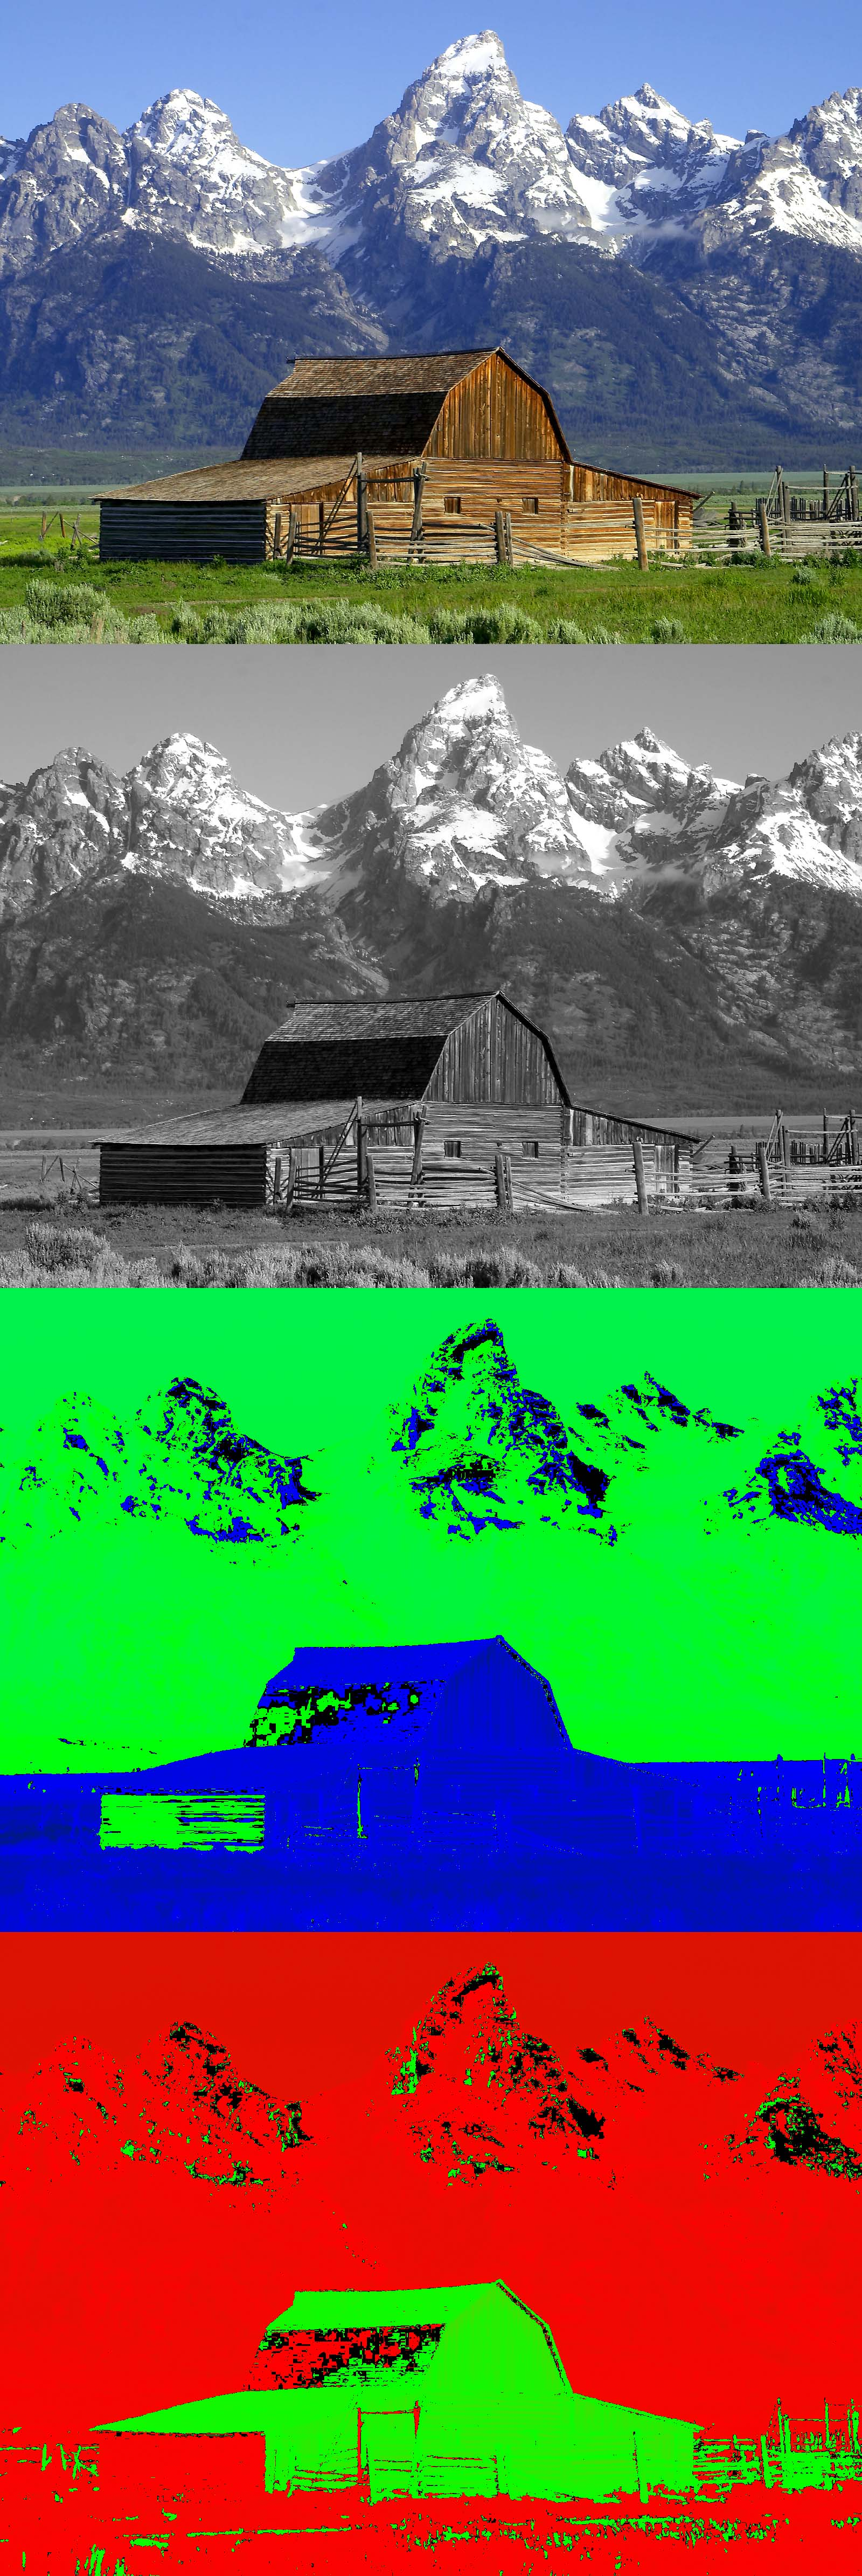
\includegraphics[height=10\baselineskip,keepaspectratio]{figures/YDbDr_components.jpg}
                \caption*{Source: \href{https://commons.wikimedia.org/wiki/File:YDbDr_components.jpg}{(3ucky(3all}, CC-BY-SA 3.0, via Wikimedia Commons}
            \end{figure}
        \end{column}
    \end{columns}
\end{frame}
\begin{frame}{Y'DbDr}
    \begin{itemize}
        \item Standardized in ITU.R BT-470.6 \parencite*{BT470}
        \item Didn't make it to its upgrade, BT.1700-0 -- obsolete
        \item Targets the \emph{D65} white point (beaten Y'CbCr!)
        \item Targets the analog domain \emph{entirely} -- no OETF or EOTF
        \item Assumes a power law $gamma = 2.2$ for the non-linearity of the display
    \end{itemize}
\end{frame}
\begin{frame}{Y'CbCr}
    \begin{columns}<.->
        \begin{column}<.->{.7\textwidth}
            \begin{itemize}
                \item Created in 1981 as a joint EBU - SMPTE standard
                \item Objective: entirely digital signal compositing pipeline
                \item $(R', G', B')$ pixel $\rightarrow$ $(Y', Cb, Cr)$ signal values
                \item $Y'$ is the \emph{luma} signal
                \item $Cb$ and $Cr$ together form the \emph{chroma} signal
                      \begin{itemize}
                          \item $Cb$ blue - luma, $Cr$ red - luma
                      \end{itemize}
                \item Key property: less than \qty{25}{\percent} of the colour space relates to valid RGB colours! \autocite{7261497}
                \item Standardized by the ITU in \emph{three} Recommendations
            \end{itemize}
        \end{column}
        \begin{column}<1->{.3\textwidth}
            \begin{figure}
                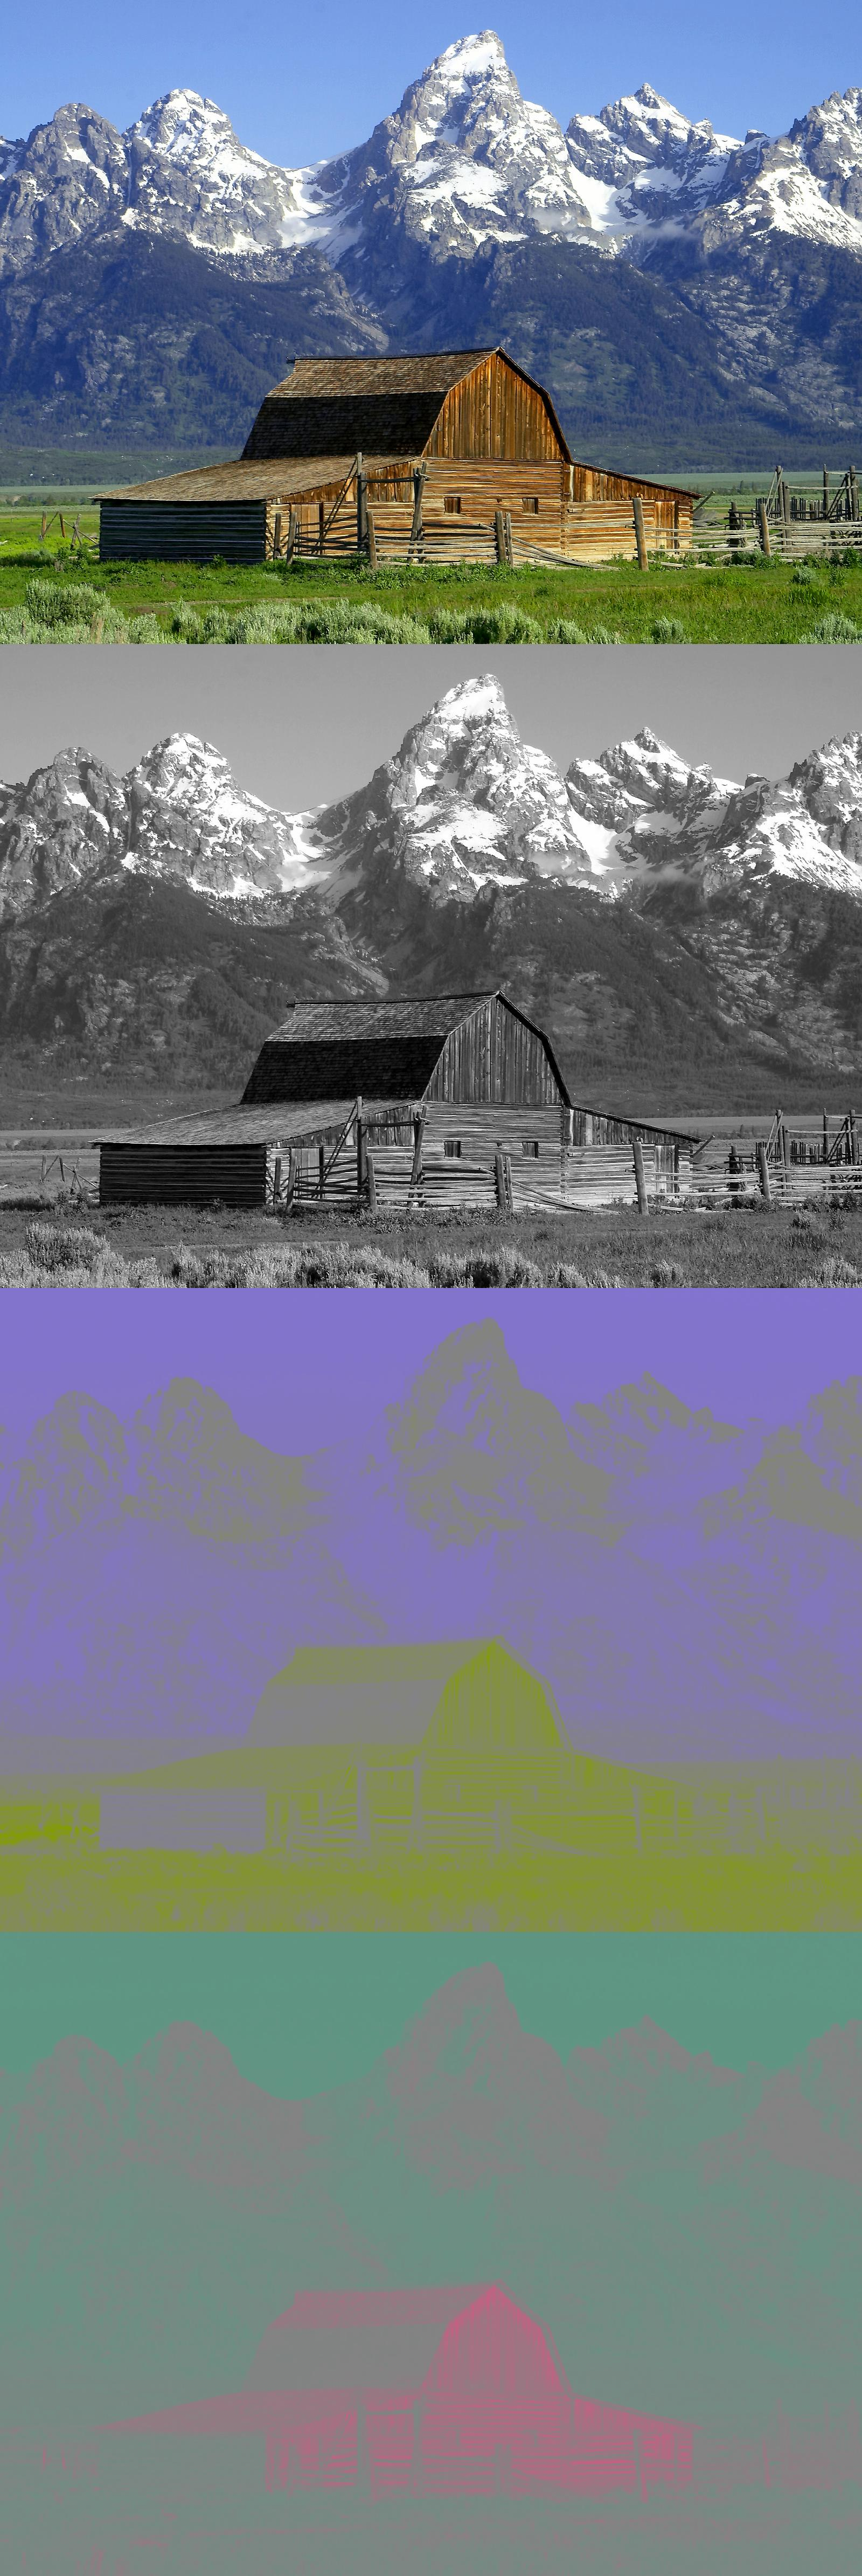
\includegraphics[height=10\baselineskip,keepaspectratio]{figures/Barns_grand_tetons_YCbCr_separation.jpg}
                \caption*{Source: \href{https://commons.wikimedia.org/wiki/File:Barns_grand_tetons_YCbCr_separation.jpg}{Mike1024}, Public domain, via Wikimedia Commons}
            \end{figure}
        \end{column}
    \end{columns}
\end{frame}
\begin{frame}{Y'CbCr: BT.601-7 (SD)}
    \begin{itemize}
        \item Last updated in \cite*{BT601}
        \item Targets standard definition transmissions ($\leq$480p)
        \item Designed for compatibility with legacy (monochrome, NTSC) receivers
        \item Targets the \emph{D65} white point
        \item Same gamma correction as Y'IQ
    \end{itemize}

    \uncover<+->{
        \begin{align}
            Y' & = 0.299R' + 0.587G' + 0.114B'                                             \\
            Cb & = \frac{0.701}{1.402}R' + \frac{-0.587}{1.402}G' + \frac{-0.114}{1.402}B' \\
            Cr & = \frac{-0.299}{1.772}R' + \frac{-0.587}{1.772}G' + \frac{0.886}{1.772}B'
        \end{align}
    }
\end{frame}
\begin{frame}{Y'CbCr: BT.709-6 (HD)}
    \begin{itemize}
        \item Last updated in \cite*{BT709}
        \item Revised version targeting HD transmissions
        \item Drops legacy compatibility in exchange for accurate eye luminance response
        \item Targets the \emph{D65} white point
        \item (Still) the same gamma correction as BT.601
    \end{itemize}

    \uncover<+->{
        \begin{align}
            Y' & = 0.2126R' + 0.7152G' + 0.0722B'                                                \\
            Cb & = \frac{-0.2126}{1.8556}R' + \frac{-0.7152}{1.8556}G' + \frac{0.9278}{1.8556}B' \\
            Cr & = \frac{0.7874}{1.5748}R' + \frac{-0.7152}{1.5748}G' + \frac{-0.0722}{1.5748}B'
        \end{align}
    }
\end{frame}
\begin{frame}{Y'CbCr: BT.2020-2 (4K/HDR)}
    \begin{itemize}
        \item Last updated in \cite*{BT2020}
        \item Revised version targeting 4K and HDR
        \item Upgraded transformation matrix and transform function
        \item Maintains the \emph{D65} white point
    \end{itemize}

    \uncover<+->{
        \begin{align}
            Y' & = 0.2627R' + 0.6780G' + 0.0593B'                                                \\
            Cb & = \frac{0.2627}{1.8814}R' + \frac{0.6780}{1.8814}G' + \frac{0.9407}{1.8814}B' \\
            Cr & = \frac{0.7373}{1.4746}R' + \frac{0.6780}{1.4746}G' + \frac{0.0593}{1.4746}B'
        \end{align}
    }
\end{frame}
\begin{frame}{Y'CbCr: gamma correction in BT.2020}
    \begin{itemize}
        \item BT.2020 defines both corrected and uncorrected versions
        \item For the sake of consistency, we cover the Y'CbCr version (gamma corrected) for 10-bit depth
        \item The OETF relates the input luminance $L$ to the electrical signal $E$: \begin{equation}
                  \small
                  E = \begin{cases}
                      (1.099L^{0.045} + 0.982) & 0.018 < L \leq 1.00 \\
                      4.500L                   & 0 \leq L \leq 0.018
                  \end{cases}
              \end{equation}
        \item The EOTF relates the electrical signal $E$ to the output luminance $L$: \begin{equation}
                  \small
                  L = \begin{cases}
                      \frac{E + 0.099}{1.099}^\frac{1}{0.4500} & 0.0812 < E \leq 1.00 \\
                      \frac{E}{4.500}                          & 0 \leq L \leq 0.0812
                  \end{cases}
              \end{equation}
    \end{itemize}
\end{frame}
\begin{frame}{sYCC}
    \begin{columns}<.->
        \begin{column}<.->{.7\textwidth}
            \begin{itemize}
                \item Standardized in 1999 as part of sRGB \autocite{srgb2002}
                \item Defines the colour space for JPEG's lossy compression step (DCT)
                \item $(R', G', B')$ pixel $\rightarrow$ $(Y', Cb, Cr)$ pixel
                \item Based on the sRGB primaries, \emph{not NTSC or BT.709}
                \item Allows extended gamut (colours that don't fit within the sRGB gamut)
            \end{itemize}
        \end{column}
        \begin{column}<1->{.3\textwidth}
        \end{column}
    \end{columns}
\end{frame}
\begin{frame}{YCgCo}
    \begin{columns}<.->
        \begin{column}<.->{.7\textwidth}
            \begin{itemize}
                \item Standardized as ITU-R H.273 \parencite*{ycocg}
                \item $(R', G', B')$ pixel $\rightarrow$ $(Y, Cg, Co)$ signal values
                      \begin{itemize}
                          \item $Cg$ and $Co$ represent \enquote{orange} and \enquote{green} chroma
                          \item \emph{Not \enquote{chrominance} as the Wikipedia page suggests!}
                      \end{itemize}
            \end{itemize}
        \end{column}
        \begin{column}<1->{.3\textwidth}
            \begin{figure}
                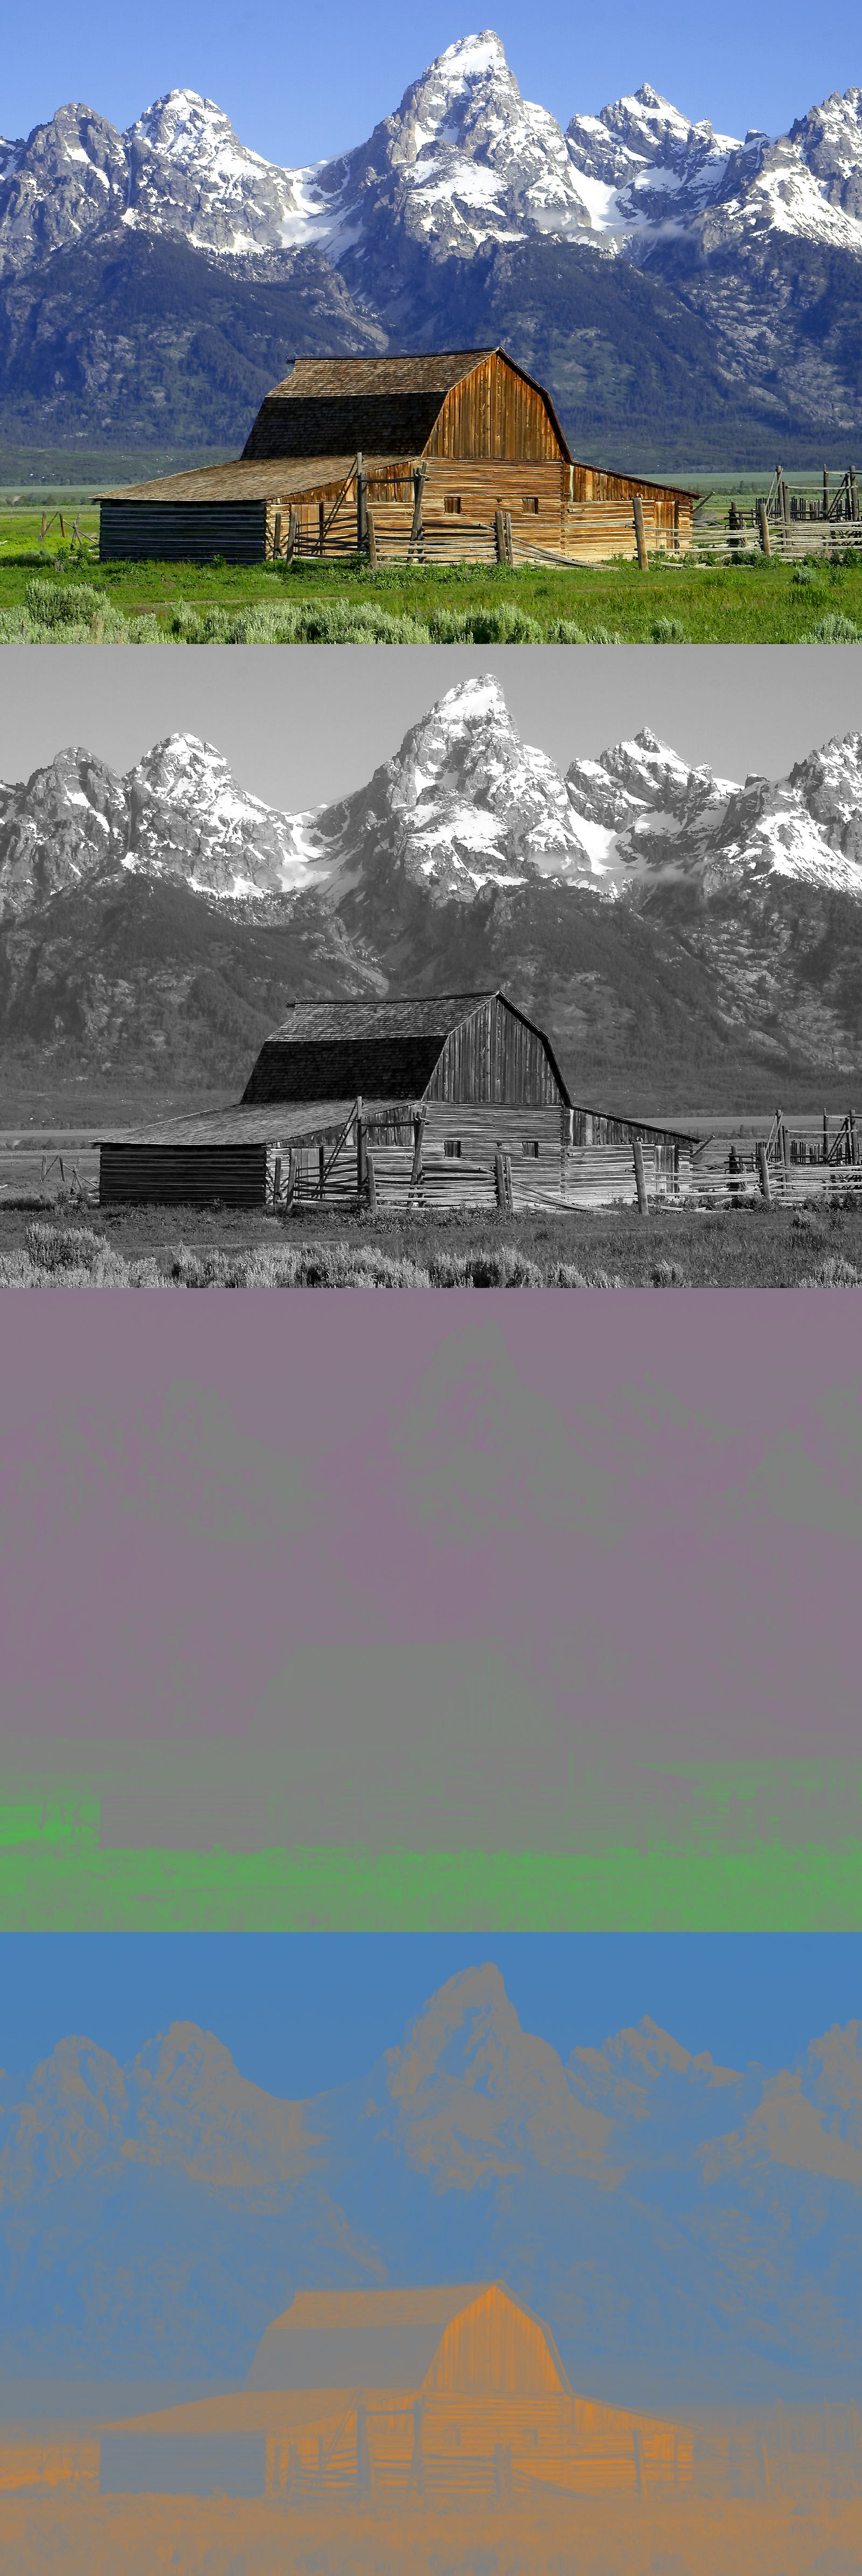
\includegraphics[height=10\baselineskip,keepaspectratio]{figures/Barns_grand_tetons_YCgCo_separation.jpg}
                \caption*{Source: \href{https://commons.wikimedia.org/wiki/File:Barns_grand_tetons_YCgCo_separation.jpg}{Devcore}, Public Domain, via Wikimedia Commons}
            \end{figure}
        \end{column}
    \end{columns}
\end{frame}

\begin{frame}{YCgCo}
    \begin{itemize}
        \item Standardized as ITU-R H.273 \parencite*{ycocg}
        \item Standard provides a single point for all transfer functions you could use!
        \item Designed for integer math -- $n+2$-bit depth is needed to preserve the full $n$-bit RGB range
    \end{itemize}

    \uncover<+->{
        \begin{align}
            \begin{bmatrix}
                Y' \\
                Cg \\
                Co
            \end{bmatrix} = \begin{bmatrix}
                                \frac{1}{4}  & \frac{1}{2} & \frac{1}{4}  \\
                                -\frac{1}{4} & \frac{1}{2} & -\frac{1}{4} \\
                                \frac{1}{2}  & 0           & -\frac{1}{2}
                            \end{bmatrix} \times \begin{bmatrix}
                                                     R' \\
                                                     G' \\
                                                     B'
                                                 \end{bmatrix}
        \end{align}
    }
\end{frame}
\begin{frame}{ICtCp}
    \begin{columns}<.->
        \begin{column}<.->{.7\textwidth}
            \begin{itemize}
                \item Designed by \textcite{ictcp}
                \item $(R', G', B')$ pixel $\rightarrow$ $(I, Ct, Cp)$ signal values
                      \begin{itemize}
                          \item Note: there's an optative linear RGB version
                      \end{itemize}
                \item $I$ is the \emph{intensity} (luma) channel
                \item $Ct$ and $Cp$ together form the \emph{chroma} channel
                      \begin{itemize}
                          \item $Ct$ is \emph{chroma tritan} (yellow-blue)
                          \item $Cp$ is \emph{chrome protan} (red-green)
                      \end{itemize}
                \item Standardized in ITU.R BT-2100 \parencite*{BT2100}
            \end{itemize}
        \end{column}
        \begin{column}<1->{.3\textwidth}
            \begin{figure}
                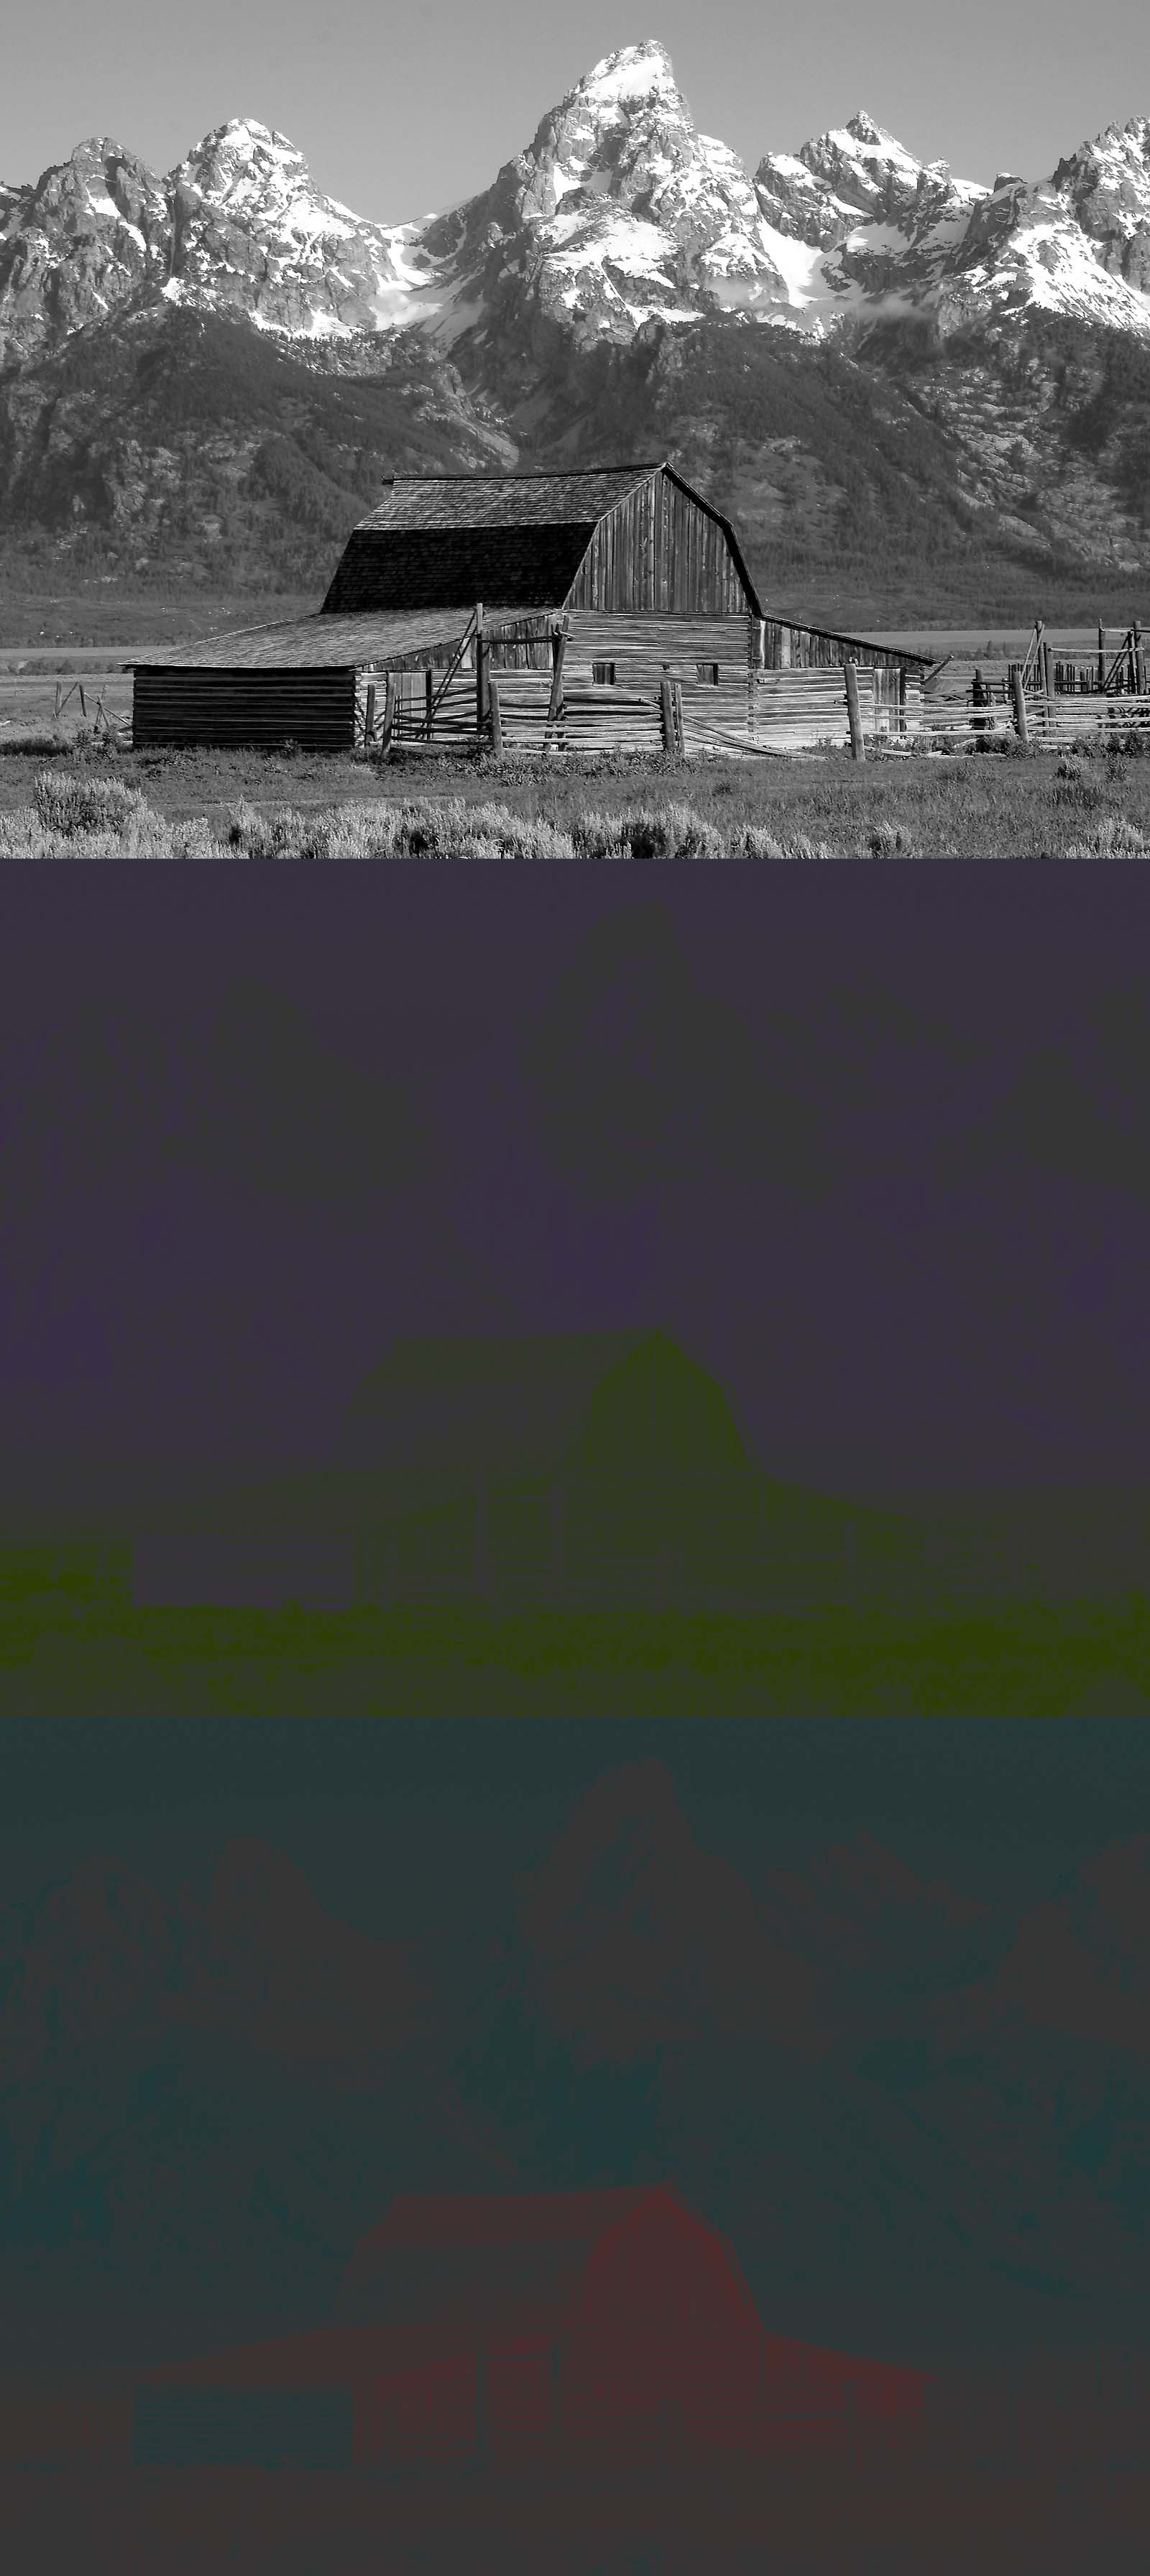
\includegraphics[height=10\baselineskip,keepaspectratio]{figures/ICtCp_components.jpg}
                \caption*{Source: based on \href{https://commons.wikimedia.org/wiki/File:Barns_grand_tetons.jpg}{Jon Sullivan (PD Photo.org)}, Public Domain, via Wikimedia Commons}
            \end{figure}
        \end{column}
    \end{columns}
\end{frame}
\begin{frame}{ICtCp}
    \begin{itemize}
        \item It is \emph{not} a linear transformation
        \item Requires a complete CMS transformation pipeline
        \item Also requires the BT.2100 transfer functions for HDR
        \item $R'G'B' \xrightarrow{OETF} RGB \to LMS \to ICtCp$
        \item Can't add more details, it'd turn this into a whole extra talk \emoji{sweat-smile}
    \end{itemize}
\end{frame}
\section{Conclusions}
\begin{frame}{Remarks}
    \begin{itemize}
        \item So many colour spaces
        \item Originally designed for analog broadcasting
        \item Now present in all everyday multimedia applications
        \item We covered
              \begin{itemize}
                  \item A primer on colour spaces
                  \item The basics of colour managements
                  \item Why are luma-chroma colour spaces so essential
                  \item Examples
              \end{itemize}
    \end{itemize}
\end{frame}
\begin{frame}{Remarks}
    \begin{itemize}
        \item We did not cover the full background behind colour spaces
        \begin{itemize}
            \item Trichromacy, $LMS$ cone response functions
        \end{itemize}
        \item We also did not cover what's needed for 4K/HDR
        \begin{itemize}
            \item YCbCr v ICtCp in digital workflows
        \end{itemize}
        \item That would make for another hour of talk!
        \item Extra references at the end of this talk's slides
    \end{itemize}
\end{frame}
\begin{frame}{Thank you for watching!}
    \begin{center}
        {
            \large
            \textbf{Got any questions or comments?}
        }

        Q+A next

        Email: \href{mailto:amy@amyspark.me?subject="FireShonks 2023"}{amy@amyspark.me}

        Matrix: \href{https://matrix.to/\#/@amyspark:fairydust.space}{@amyspark:fairydust.space}
    \end{center}
\end{frame}
% https://tex.stackexchange.com/questions/30461/beamer-nonumber-equivalent-for-slides
\begin{frame}[plain,noframenumbering,allowframebreaks]{\bibname}
    \printbibliography[heading=none]
\end{frame}
\end{document}
